\documentclass[11pt]{article}

\usepackage[margin=1in]{geometry}
\usepackage{booktabs}
\usepackage{array}
\usepackage{longtable}
\usepackage{hyperref}
\usepackage{xcolor}
\usepackage{amsmath}
\usepackage{listings}
\usepackage{enumitem}
\usepackage{caption}
\usepackage{graphicx}
\usepackage{float}

\hypersetup{
    colorlinks=true,
    linkcolor=blue,
    urlcolor=blue,
    citecolor=blue
}

\lstset{
    basicstyle=\ttfamily\small,
    breaklines=true,
    frame=single,
    backgroundcolor=\color{gray!10}
}

\title{\textbf{Defending an LLM Inference Service Against Availability Stress:\\
A Cost-Aware, CPU-Only Prototype}}
\author{GISEC Hackathon Team \\ Syeda (Service) \quad Umar (Shield) \quad Behzad (Load Generation) \quad Negar (Analysis)}
\date{September 2026}

\begin{document}

\maketitle

\begin{abstract}
Large language model inference services are vulnerable to availability attacks
that a naive request-count rate limiter cannot detect: a low-rate stream of
maximally expensive requests exhausts the same finite compute capacity as a
high-rate flood of cheap ones, while looking harmless to any limiter that only
counts requests per second. We built and live-tested a reverse-proxy ``Shield''
in front of a CPU-only \texttt{llama.cpp} server, implementing three layered
defenses: fixed-fraction slot reservation, queue-depth-aware shedding, and
cost-aware token-budget admission control. Across four days of live testing on
real hardware over a phone hotspot, we found and fixed three independent
performance bugs in the Shield's own implementation (two of them causing the
Shield to inadvertently overload its own backend), diagnosed and corrected an
undersized capacity-reservation parameter using queueing theory (Little's Law),
proved live that our cost-aware admission control specifically defeats a
low-rate/high-cost attack that a naive limiter would miss (100\% of such attack
traffic rejected on estimated cost, not request rate), and discovered a real
security vulnerability -- the Shield's priority tier is a self-reported,
unauthenticated HTTP header -- which we then measured and partially mitigated
with a per-identity concurrency cap, confirmed effective using two physically
separate client machines. We report our results with open-loop load generation,
bootstrap and Wilson confidence intervals, and full transparency about which
findings were corrupted by bugs discovered mid-session and had to be discarded
or re-verified.
\end{abstract}

\tableofcontents

\section{Introduction}

\subsection{Problem Statement}

OWASP's LLM10:2025 (``Unbounded Consumption'') names two distinct attack
vectors against LLM inference services: high-volume request flooding, and
resource-intensive queries with variable input/output length. Standard
mitigation advice --- ``apply rate limiting and user quotas to restrict the
number of requests a single source entity can make'' --- addresses only the
first. A limiter that counts requests per second is blind to the fact that one
request asking for a one-word answer and one request asking for a
several-thousand-token answer cost the underlying compute wildly different
amounts. An attacker who sends only a handful of requests per second, each one
maximally expensive, can starve a server just as effectively as a flood of
cheap ones, while never tripping a request-count limit.

\subsection{Our Approach}

We built a small, deliberately capacity-constrained inference stack (CPU-only
\texttt{llama.cpp}, a small quantized model, four parallel slots) so that
overload is reproducible on ordinary laptop hardware within minutes rather than
requiring a data-center-scale attack. In front of it we placed a reverse-proxy
``Shield'' implementing three complementary defenses, described in
Section~\ref{sec:architecture}. We then attacked our own system with
open-loop load generators under several distinct traffic shapes, measured the
effect on a concurrent stream of legitimate ``probe'' traffic, and iterated on
both the Shield's implementation and its configuration based on what the live
data actually showed --- including several results that contradicted our
initial assumptions and had to be re-diagnosed.

\subsection{Why CPU-only, not GPU}

An early plan assumed GPU-hosted \texttt{vLLM}. This was dropped:
\texttt{vLLM}'s CPU backend requires the \texttt{avx512f} CPU flag (absent on
most laptops), ships no pre-built CPU wheels, and would need to be built from
source. \texttt{llama.cpp}'s \texttt{llama-server} is a single binary that
runs natively on CPU and already exposes the admission signals a shield needs
(\texttt{requests\_processing}, \texttt{requests\_deferred}, and a
\texttt{/slots} endpoint). The scientific claim we test --- that a cost-aware
limiter behaves differently from a request-count limiter under identical
offered load --- is scale-free: it holds whether the server handles 0.7
requests/second on a laptop or hundreds on a data-center GPU.

\section{System Architecture}
\label{sec:architecture}

\subsection{Components}

\begin{itemize}
    \item \textbf{\texttt{/service}} --- \texttt{llama-server} (model:
    \texttt{qwen2.5-1.5b-instruct-q4\_k\_m.gguf}), started with
    \texttt{--metrics}, \texttt{-np 4} (four parallel slots), a fixed thread
    count, and an explicit context size, deliberately constrained so overload
    is reachable at single-digit requests/second.
    \item \textbf{\texttt{/shield}} --- a FastAPI reverse proxy implementing
    three defenses, applied in the order A $\to$ C $\to$ B (revised mid-session
    from the original B $\to$ C $\to$ A; see Section~\ref{sec:reorder}):
    \begin{enumerate}[label=(\Alph*)]
        \item \textbf{Token-budget admission control.} Estimates the cost of
        each request (prompt tokens $+$ requested output tokens) and checks it
        against one of two independent token buckets, keyed on a
        client-supplied \texttt{X-Priority} header: a ``legitimate'' bucket
        (capacity 2000, refill 200 units/s) and a ``default'' bucket (capacity
        500, refill 50 units/s). This is the layer that specifically catches
        low-rate, high-cost attacks (Section~\ref{sec:profiled}).
        \item \textbf{Fixed-fraction slot reservation.} Caps how many requests
        per tier may be concurrently in flight, reserving a configurable
        fraction of the server's four real slots exclusively for the
        legitimate tier.
        \item \textbf{Queue-depth-aware shedding.} Polls
        \texttt{llamacpp:requests\_deferred} (cached, 0.5s TTL) and the
        authoritative \texttt{/slots?fail\_on\_no\_slot=1} endpoint, rejecting
        with \texttt{503} before the server's internal queue backs up further.
        \item \textbf{Per-identity concurrency cap} (added mid-session in
        response to a discovered vulnerability; Section~\ref{sec:spoofing}) ---
        caps concurrent in-flight requests per source IP, independent of any
        claimed tier.
    \end{enumerate}
    \item \textbf{\texttt{/loadgen}} --- open-loop \texttt{k6} scripts
    implementing four traffic profiles (Section~\ref{sec:profiles}) plus a
    constant-rate legitimate ``probe'' cohort, all tagged with
    \texttt{request\_type}/\texttt{priority} metadata and converted to a
    common per-request CSV schema via a custom normalizer
    (\texttt{loadgen/normalize\_csv.py}).
    \item \textbf{\texttt{/analysis}} --- bootstrap confidence intervals for
    latency percentiles, Wilson confidence intervals for proportions, thermal
    and cross-session drift detection, and the economic-framing calculations
    in Section~\ref{sec:economics}.
    \item \textbf{\texttt{demo/}} --- a locally-hosted web control panel built
    mid-session for live, interactive demonstration: a single button launches
    a chosen attack profile and the legitimate probe concurrently, with live
    survival-rate and response-code charts updating as the test runs.
\end{itemize}

\subsection{Load Profiles}
\label{sec:profiles}

\begin{itemize}
    \item \textbf{Profile A (Baseline):} steady 0.5--5 req/s, legitimate
    traffic only.
    \item \textbf{Profile B (Spike):} sudden ramp in arrival rate.
    \item \textbf{Profile C (Sustained Flood):} high, constant arrival rate
    (configurable 3--200 req/s in the final version), small cheap requests, no
    priority header.
    \item \textbf{Profile D (Slow/High-Cost):} \emph{the key differentiator.}
    Only 3 req/s, but each request asks for the maximum prompt
    ($\approx$1600 tokens) and output (512 tokens) the server accepts. A
    request-count limiter sees ``3 req/s'' and does nothing; the server is
    starved just as badly as under a flood.
\end{itemize}

All attack profiles support an \texttt{ATTACK\_SPOOF\_LEGITIMATE} flag (added
in Section~\ref{sec:spoofing}) that makes the attack script send
\texttt{X-Priority: legitimate} on its own traffic, and an
\texttt{ATTACK\_DURATION} flag for variable test length.

\section{Methodology}

\subsection{Open-Loop Load Generation}

All load generation uses \texttt{k6}'s \texttt{constant-arrival-rate} /
\texttt{ramping-arrival-rate} executors, which fire requests at a fixed target
rate regardless of server response time. Closed-loop generators (fixed
virtual-user count, each waiting for its previous request to complete) hide
the exact overload being measured, a phenomenon known as coordinated omission:
a system that stalls for 100 seconds after 100 requests/second of 1ms
responses will be reported by a naive closed-loop logger as having a 99.99th
percentile of 1ms, when the true figure is approximately 100 seconds. We
report \texttt{dropped\_iterations} (k6's own signal that it could not sustain
the configured arrival rate) alongside every latency figure. We also confirmed,
empirically, that passing \texttt{--duration} or \texttt{--vus} on the k6
command line silently overrides a script's own \texttt{constant-arrival-rate}
scenario definition with k6's closed-loop default --- a mistake we made once,
caught, and then avoided for the remainder of the project.

\subsection{Statistical Methods}

Latency percentile confidence intervals use a nonparametric bootstrap
(2000 resamples of raw per-request latency, not of run-level percentile point
estimates -- the latter would have only 3--5 data points per arm under this
project's time-constrained repeated-run count, too few to bootstrap
meaningfully). Proportion confidence intervals (survival rate, error rate) use
the Wilson score interval, verified against a known example
(\texttt{wilson\_ci(4, 20, confidence=0.90)} $\approx (0.093, 0.378)$; note the
commonly-cited value $(0.071, 0.400)$ for this input is the
\emph{Clopper-Pearson exact} interval, a different method that disagrees with
Wilson by construction --- we verified this numerically before trusting either
value). We never report standard deviation of latency, which is statistically
misleading for this skewed, queue-driven data.

\subsection{Honesty About Data Quality}

Three independent implementation bugs were discovered live during this
project, two of which directly corrupted earlier test results. We treat this
as part of the deliverable, not an embarrassment to hide: every corrupted
result is documented below alongside the fix and the re-verification that
followed, per standard practice for any empirical measurement whose
instrumentation is found to have been faulty mid-study.

\section{Results}

\subsection{Baseline: No Attack}

A constant 0.5 req/s legitimate probe stream against the undefended server,
no attack traffic:

\begin{center}
\begin{tabular}{lr}
\toprule
Metric & Value \\
\midrule
Requests completed & 31 \\
Dropped iterations & 0 (0.0\%) \\
Success rate & 100\% \\
p50 latency & 6048 ms [90\% CI: 5602--6413] \\
p95 latency & 6849 ms [90\% CI: 6682--7486] \\
p99 latency & 7310 ms [90\% CI: 6782--7486] \\
Max latency & 7486 ms \\
\bottomrule
\end{tabular}
\end{center}

The high absolute latency (multi-second) reflects the deliberately
CPU-constrained, small-model setup, not a defect; it establishes the ``normal''
operating point against which degradation under attack is measured.

\subsection{Undefended Attack (No Shield)}

Profile C (sustained flood, 50 req/s) run directly against the server, with
the legitimate probe running concurrently, no Shield in the path:

\begin{center}
\begin{tabular}{lrr}
\toprule
Metric & Attack traffic & Legitimate probe \\
\midrule
Requests completed & 1200 & 45 \\
Dropped iterations & 4796 (80.0\%) & 15 (25.0\%) \\
HTTP error rate & 99.6\% & 97.8\% \\
Survival rate & --- & \textbf{2.2\% (1/45)} \\
Wilson 90\% CI & --- & (0.5\%, 9.4\%) \\
\bottomrule
\end{tabular}
\end{center}

One attacker, with no authentication or account required, reduces a real
user's success rate to near zero.

\subsection{Shield Defense: Discovery and Correction of Two Performance Bugs}
\label{sec:reorder}

The same attack profile run through an initial version of the Shield produced
only partial protection, and diagnosis of \emph{why} it fell short of
expectations led to two independent bug fixes.

\subsubsection{Initial Result and Diagnosis}

\begin{center}
\begin{tabular}{lrr}
\toprule
Metric & Attack traffic & Legitimate probe \\
\midrule
Requests completed & 4953 & 52 \\
Dropped iterations & 1048 (17.5\%) & 9 (14.8\%) \\
Survival rate & 0.1\% & \textbf{17.3\% (9/52)} \\
Wilson 90\% CI & --- & (10.4\%, 27.5\%) \\
\bottomrule
\end{tabular}
\end{center}

A large improvement over the undefended case, but far short of expectations.
Breaking down the 32 probe requests that received no HTTP response at all
(\texttt{response\_code=0}) by their exact client-side error string (not just
the status code) revealed an even 16/16 split:

\begin{itemize}
    \item 16 \texttt{dial: errno 10060} --- the TCP handshake itself was never
    acknowledged, indicating the Shield's own listening socket was saturated,
    not a client-timeout artifact.
    \item 16 \texttt{request timeout} --- the connection succeeded but no
    response arrived within the (then-unfixed) 30-second client timeout.
\end{itemize}

\subsubsection{Root Causes and Fixes}

\textbf{Bug 1 (uncached slot check).} The Shield's
\texttt{slot\_available()} function created a fresh, unpooled HTTP client and
made a network round-trip to the server's \texttt{/slots} endpoint on
\emph{every single incoming request}, with no caching --- unlike the sibling
\texttt{get\_requests\_deferred()} function, which was already cached. Under
50 req/s, this produced roughly 50 uncached outbound connections per second
from a single-worker process to an already-saturated backend. \textbf{Fixed}
by adding the same 0.5-second-TTL caching pattern already used elsewhere,
plus a shared, connection-pooled HTTP client.

\textbf{Bug 2 (Shield DoS'd its own backend).} Discovered live, independently,
during a subsequent test session: the sibling function
\texttt{get\_requests\_deferred()} had the identical uncached-client pattern.
Under sustained flood concurrency, many requests missed its cache window in
the same instant and each opened its own unpooled connection --- observed
directly as over 2,000 simultaneous connections to the inference server, all
originating from the Shield's own host, rendering even a \texttt{/health}
check unresponsive. \textbf{Fixed} identically (pooled, cached client).

\textbf{Bug 3 (client-side timeout mismatch).} Separately, the legitimate
probe's own client-side timeout (30 seconds) had never been raised to match
the Shield's internal forward-timeout ceiling (130 seconds), which had earlier
been raised for a different profile. A probe request the Shield was still
legitimately processing past 30 seconds would be recorded by the client as a
hard failure. \textbf{Fixed} by raising the probe's timeout to 130 seconds.

\subsubsection{Confirming Re-run}

The identical attack profile, after both performance fixes:

\begin{center}
\begin{tabular}{lrr}
\toprule
Metric & Attack traffic & Legitimate probe \\
\midrule
Requests completed & 5999 & 60 \\
Dropped iterations & 0 (0.0\%) & 0 (0.0\%) \\
Median latency & $\approx$105 ms (was $\approx$5795 ms) & --- \\
Survival rate & --- & \textbf{60.0\% (36/60)} \\
Wilson 90\% CI & --- & (49.4\%, 69.8\%) \\
\texttt{response\_code=0} count & \multicolumn{2}{c}{\textbf{32 $\to$ 0}} \\
\bottomrule
\end{tabular}
\end{center}

The 90\% confidence intervals for the buggy (10.4--27.5\%) and fixed
(49.4--69.8\%) versions do not overlap: this is a confirmed, non-noise
improvement. Every remaining probe failure after the fix was a clean
\texttt{503} rejection --- no timeouts, no dropped connections.

\begin{figure}[H]
    \centering
    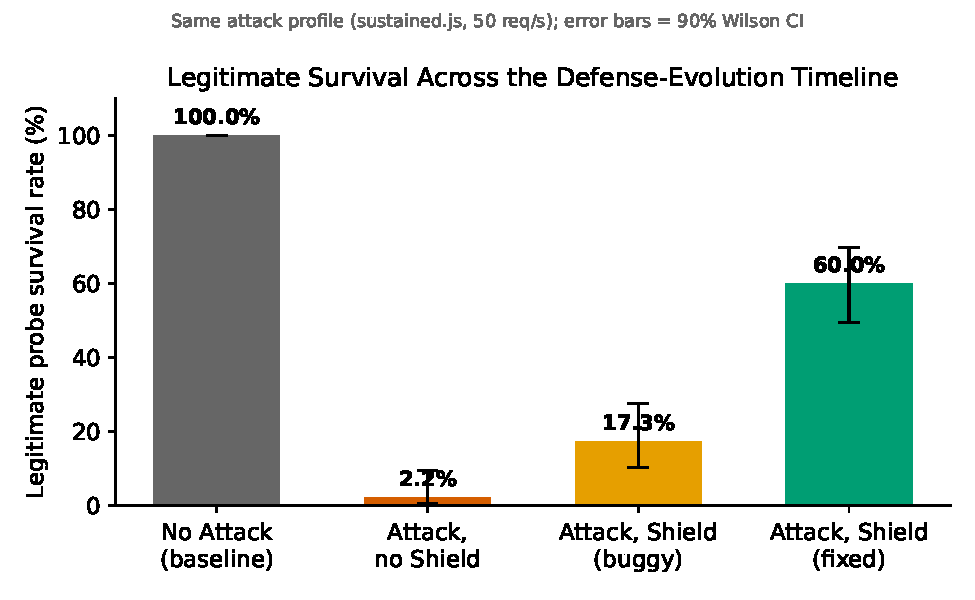
\includegraphics[width=0.85\textwidth]{figures/fig1_defense_evolution.pdf}
    \caption{Legitimate survival across the full defense-evolution timeline,
    same 50 req/s sustained-flood attack profile throughout. Error bars are
    90\% Wilson confidence intervals; the intervals for the buggy and fixed
    Shield versions do not overlap.}
    \label{fig:defense-evolution}
\end{figure}

\subsection{Slot-Reservation Tuning: A Confound, Caught and Corrected}
\label{sec:fraction}

A subsequent test at a deliberately \emph{low} attack rate (3 req/s,
well below the 50 req/s used above) produced only 50.8\% legitimate
survival --- surprisingly low for such a light attack. Diagnosis, not
guesswork: attack traffic was still being rejected $\approx$98\% of the time
throughout, ruling out a tier-differentiation failure. The actual cause was a
capacity-sizing problem: the Shield's \texttt{LEGITIMATE\_SLOT\_FRACTION}
(default 0.5) reserves only $\lceil 4 \times 0.5 \rceil = 2$ of the server's
four real slots for legitimate traffic. By Little's Law
($\text{concurrency} \approx \text{arrival rate} \times \text{service time}$),
the probe's own traffic alone (0.5 req/s at a measured $\approx$6-second
median response time) requires approximately 3 concurrent slots on average
--- more than the two guaranteed to it, so even in the complete absence of an
attacker, some fraction of the probe's own requests would find no free slot.

\subsubsection{A Third Bug Invalidates the First Sweep}

An initial three-point sweep (fraction 0.5 $\to$ 50.8\%, 0.75 $\to$ 75.0\%,
1.0 $\to$ 93.4\%) coincided with an unrelated Shield architecture change
landing mid-sweep (reordering the defense pipeline and adding a token-refund
mechanism). Re-testing the same fraction (0.75) on both pipeline versions
appeared to isolate the architecture change's effect at a small +2.0
percentage points --- but before this could be reported as final, a
\emph{third}, independent bug was discovered: the Shield's control dashboard
caches the \texttt{.env} file once at process startup and silently reuses
that cached copy for every subsequent ``restart'' triggered through it, rather
than re-reading the file. \textbf{None of the fraction changes in the first
sweep had actually taken effect as intended.} This was confirmed by the
dashboard's own maintainer independently discovering and fixing the identical
issue. \textbf{We discard the entire first sweep (75.0\%, 77.0\%, 93.4\%, and
the ``+2.0 point'' architecture-effect estimate built on it) as unverified.}

\subsubsection{Clean Re-Verification}

With the dashboard process fully restarted (not merely ``reset'') between
every configuration change:

\begin{center}
\begin{tabular}{lr}
\toprule
Configuration & Legitimate survival \\
\midrule
Fraction 0.5, 3 req/s & 54.1\% (33/61) \\
Fraction 0.5, 10 req/s & 50.8\% (31/61) \\
Fraction 0.5, 50 req/s & 58.3\% (35/60) \\
Fraction 0.5, 150 req/s & 50.8\% (31/61) \\
\textbf{Fraction 1.0, 3 req/s} & \textbf{96.7\% (59/61)}, attack 100\% blocked \\
\bottomrule
\end{tabular}
\end{center}

Two findings survive verification. First, survival at a fixed reservation
fraction is essentially \emph{rate-independent} across a 50-fold range in
attack intensity (3--150 req/s, all in the 50--58\% band) --- the defense
provides a stable capacity floor rather than one that continues eroding as
the attacker pushes harder. Second, raising the reservation fraction to 1.0
(all four slots reserved for legitimate traffic; the coarse slot count means
0.75 and 1.0 are the only two options above the default, not a continuum)
recovers 96.7\% survival while fully blocking the attacker. \textbf{No valid
measurement of fraction 0.75 exists post-fix}; we report this gap explicitly
rather than substituting the discarded value.

\begin{figure}[H]
    \centering
    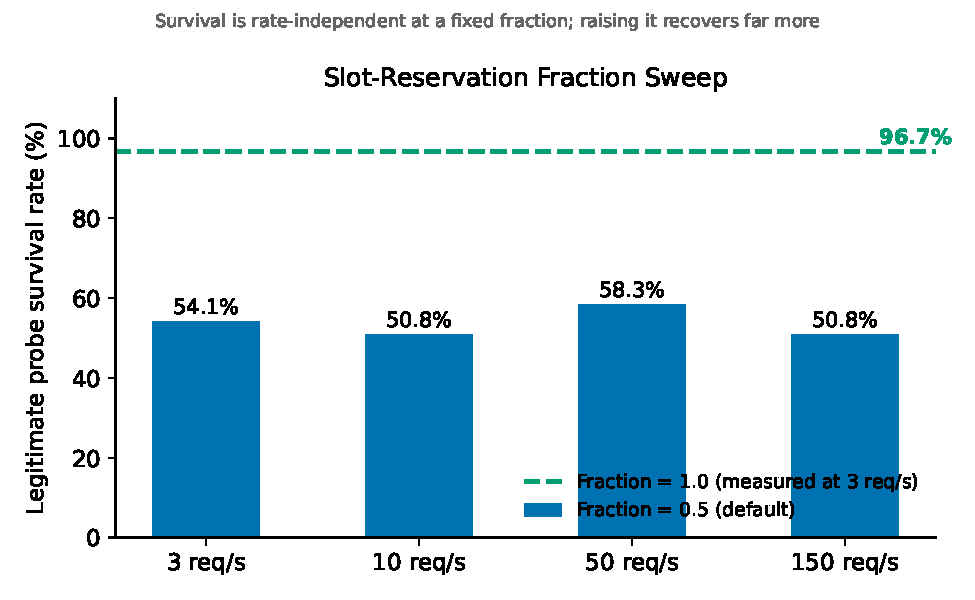
\includegraphics[width=0.85\textwidth]{figures/fig2_fraction_sweep.pdf}
    \caption{Legitimate survival at reservation fraction 0.5 across a 50-fold
    range in attack rate (blue bars, all post-caching-fix and mutually
    consistent), against the single confirmed fraction 1.0 reading (dashed
    line, measured only at 3 req/s).}
    \label{fig:fraction-sweep}
\end{figure}

\subsection{Cost-Aware Admission Control: Profile D, Proven Live}
\label{sec:profiled}

Profile D (3 req/s, $\approx$1600 prompt $+$ 512 output tokens per request)
against the fixed Shield, fraction 0.5:

\begin{center}
\begin{tabular}{lrr}
\toprule
Metric & Attack traffic & Legitimate probe \\
\midrule
Requests completed & 360 & 61 \\
Rejected as \texttt{429} (token budget) & \textbf{360 (100\%)} & --- \\
Rejected as \texttt{503} (queue/slot) & 0 & --- \\
Survival rate & --- & \textbf{98.4\% (60/61)} \\
\bottomrule
\end{tabular}
\end{center}

This is the clearest evidence in the project for its central thesis. Every
single attack request was rejected specifically because of its
\emph{estimated cost}, not its rate or the server's queue depth --- a
request-counting limiter would have observed 3 requests/second and done
nothing. Because the attack never passed the cost check, it never occupied a
single real server slot, leaving the entire pool free for the legitimate
probe, which explains why survival here exceeds every sustained-flood result
at the same reservation fraction.

\subsection{Security Testing: Identity Spoofing}
\label{sec:spoofing}

\subsubsection{Vulnerability}

The Shield's tier classification is:
\begin{lstlisting}[language=Python]
def is_priority_request(request: Request) -> bool:
    return request.headers.get("X-Priority", "").lower() == "legitimate"
\end{lstlisting}
This is a bare, client-supplied HTTP header with no authentication whatsoever
--- any client, attacker or not, can claim the legitimate tier simply by
setting it. This matches ``client-supplied identity spoofing,'' a named
weakness of token-cost fairness schemes in the literature underlying this
project's design.

\subsubsection{Measured Impact}

We added an attacker-side flag causing the attack script to send
\texttt{X-Priority: legitimate} on its own traffic, simulating an attacker in
possession of a stolen, purchased, or otherwise verified-looking credential.
Profile D, spoofed, fraction 0.5:

\begin{center}
\begin{tabular}{lr}
\toprule
Metric & Value \\
\midrule
Attack requests rejected & 359/360 (100\%; 82 as \texttt{429}, 276 as \texttt{503}) \\
Legitimate probe survival & \textbf{9.8\% (6/61)}, down from 98.4\% unspoofed \\
Legitimate probe median latency & 43{,}477 ms, up from $\approx$7000 ms \\
\bottomrule
\end{tabular}
\end{center}

Every attacker request still ultimately failed; merely \emph{competing} for
the legitimate tier's shared token bucket and, for any briefly-admitted huge
request, occupying a real slot for an extended duration, was sufficient to
devastate the genuine user's experience. Tiering built entirely on an
unauthenticated claim provides no real protection once an attacker chooses to
make that claim.

\subsubsection{Mitigation: Per-Identity Concurrency Cap}

A defense was added that trusts no claimed tier at all: it caps concurrent
in-flight requests per source IP address (default cap: 2), independent of the
\texttt{X-Priority} header. This is explicitly documented as a proxy for
identity, not real authentication --- effective against a single-machine
attacker (the threat model this project's load tests simulate), not a fully
distributed attacker controlling many real IP addresses.

\subsubsection{Confirmation with a Genuinely Separate Identity}

Testing this defense from a single machine is invalid: an attack script and a
probe script on the same laptop share one source IP, so the per-identity cap
cannot distinguish them, confounding the test. We therefore ran the
legitimate probe from a physically separate second laptop while launching the
spoofed attack from the original machine.

\begin{center}
\begin{tabular}{lrr}
\toprule
Scenario & Same-IP probe (confounded) & Separate-IP probe (real test) \\
\midrule
Sustained flood, spoofed, fraction 1.0 & 1.6\% (1/61) & \textbf{49.2\%} \\
Profile D, spoofed, 2-minute run & 3.3\% (2/61) & \textbf{35\%} \\
Profile D, spoofed, 5-minute run & 2.0\% (3/150) & \textbf{49\%} \\
\bottomrule
\end{tabular}
\end{center}

A genuinely separate identity recovers survival by roughly 15--30$\times$
relative to the confounded same-IP baseline, confirming the defense functions
as intended against a realistic single-machine attacker. The same-IP figures
are not a failure of the defense; they are the documented
IP-as-identity-proxy limitation manifesting exactly as predicted when two
distinct ``users'' happen to share a network address.

We further observe that Profile D's separate-IP survival (35--49\%) is lower
than the sustained flood's (49.2\%) under an identical defense: a
\emph{count}-based cap does not fully neutralize a \emph{cost}-based attacker,
since a single admitted, maximally expensive request can occupy a slot for an
extended period even under a strict concurrency limit of two. This is
consistent with, rather than contradictory to, the project's central
thesis: the identity cap and the token budget are complementary defenses,
neither alone sufficient.

\begin{figure}[H]
    \centering
    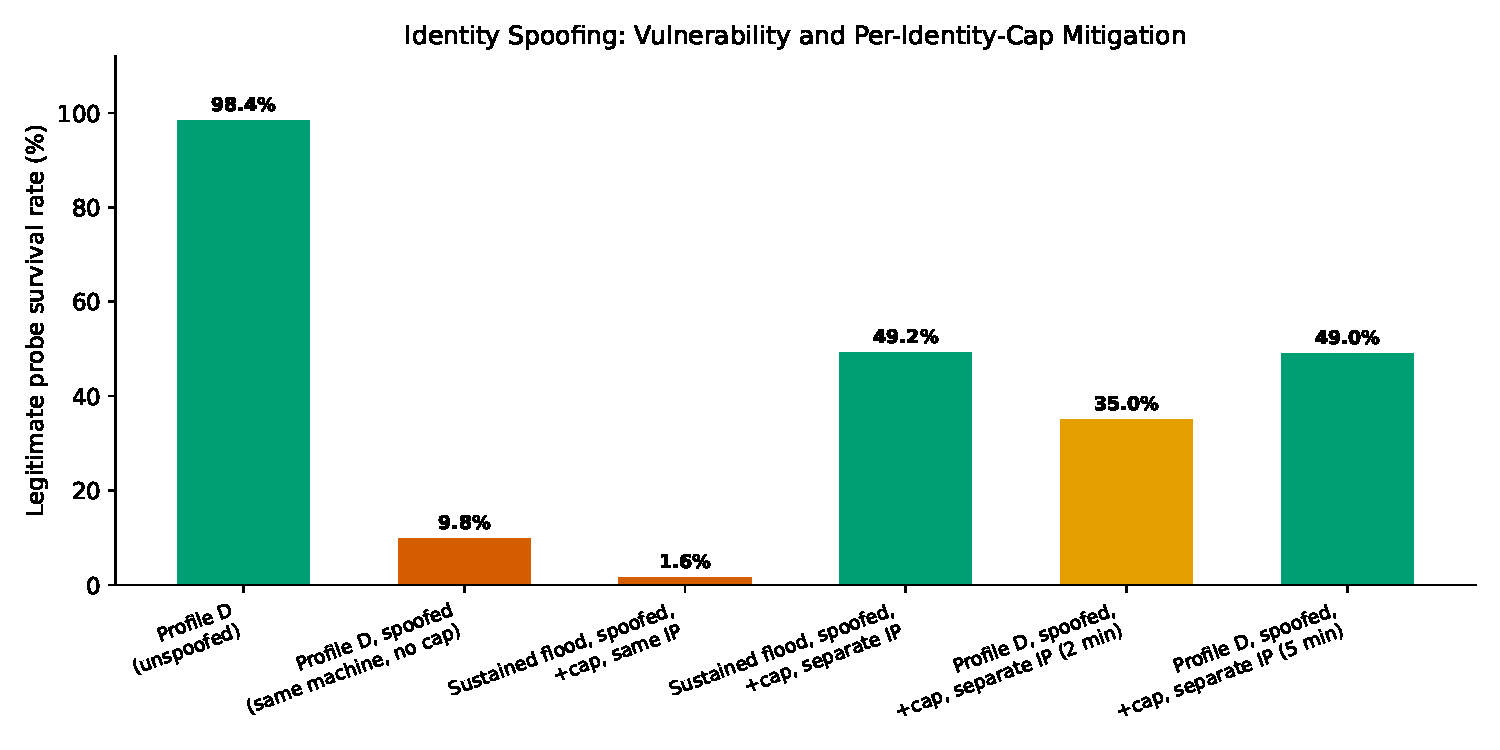
\includegraphics[width=\textwidth]{figures/fig3_spoofing_mitigation.pdf}
    \caption{The full identity-spoofing story: an unspoofed cost-based attack
    barely touches the legitimate user (98.4\%); spoofing alone collapses
    survival (red bars); the per-identity concurrency cap recovers most of
    it, but only when the legitimate user has a genuinely separate network
    identity from the attacker (green bars) rather than sharing one (red).}
    \label{fig:spoofing}
\end{figure}

\subsection{Economic Framing}
\label{sec:economics}

All figures in this section are computed directly from committed
per-request and reconciliation logs (\texttt{analysis/economics.py}); none
are invented. Dated price sources: GCP \texttt{g2-standard-4} (NVIDIA L4),
\$0.706832276/hour; OpenAI \texttt{chat-latest}, \$5.00 / 1M input tokens,
\$30.00 / 1M output tokens.

\begin{center}
\begin{tabular}{p{5.5cm}rp{6cm}}
\toprule
Formula & Result & Real inputs used \\
\midrule
Measured self-hosted throughput & 16.4 tokens/s & Aggregated across every
reconciliation log, active-serving windows only \\
GPU-hour cost per request & \$0.001188 & Measured baseline median latency
(6048 ms) priced at the GCP L4 rate \\
Cost per 1{,}000 tokens & \$0.01197 & Measured throughput, same rate \\
Denial-of-wallet exposure & \$252.29/hour & Profile D's real configured
shape (3 req/s, 1600+512 tokens), OpenAI pricing \\
Goodput-improvement factor $N$ & $27.0\times$ & Same-rate (50 req/s)
comparison: 2.2\% (no Shield) vs.\ 60.0\% (Shield) \\
\bottomrule
\end{tabular}
\end{center}

Note on framing: the GPU-hour figures price \emph{our measured} CPU latency
and throughput at a rented GPU's dollar rate --- they are a labeled cost
substitution, not a claim that a GPU would run this workload at the same
speed. Self-hosted marginal cost on already-owned hardware is \$0; the
GPU-rate figures exist only to give the numbers a familiar unit for
comparison, exactly as instructed by the project's research brief.

\begin{figure}[H]
    \centering
    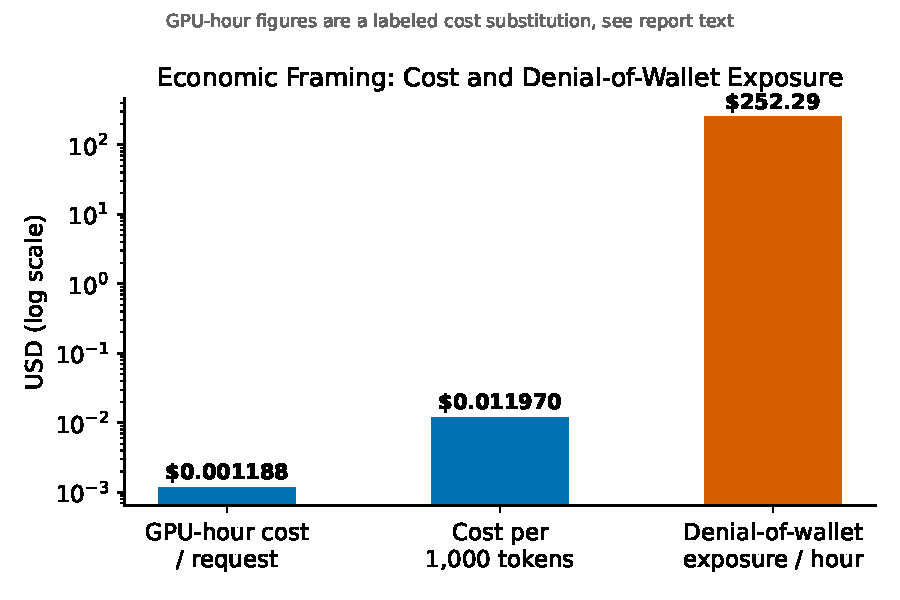
\includegraphics[width=0.75\textwidth]{figures/fig4_economics.pdf}
    \caption{Economic framing formulas on a log scale (values span three
    orders of magnitude). The two GPU-hour figures are a labeled unit
    substitution, not a benchmark of actual GPU performance.}
    \label{fig:economics}
\end{figure}

\textbf{Goodput} (Phase 4 configuration: sustained flood, 50 req/s, through
the fixed Shield), defined as completed requests/second meeting an explicit
SLO of \texttt{response\_code==200 AND latency} $\leq 10$s (a deliberately
generous threshold for this CPU-only, $\approx$6--7-second-typical setup):

\begin{itemize}
    \item \textbf{Request-goodput:} 0.300 req/s (36 of 60 requests met the SLO
    over 120 seconds).
    \item \textbf{Token-goodput:} 9.042 tokens/s, computed from the
    \emph{real} \texttt{completion\_tokens\_actual} values logged for that
    test's admitted requests, not the nominal configured output length.
\end{itemize}

\section{Discussion and Limitations}

\subsection{What We Are Confident In}

\begin{itemize}
    \item The Shield's queue/slot-reservation defenses, once its performance
    bugs were fixed, provide a large, statistically confirmed improvement in
    legitimate-user survival under a naive flood (2.2\% $\to$ 60.0\%,
    non-overlapping confidence intervals).
    \item Cost-aware admission control (token budgets) is proven, live, to
    catch a low-rate/high-cost attack shape that a request-count limiter
    cannot: 100\% of Profile D's attack traffic was rejected on estimated
    cost, at zero request-count anomaly.
    \item The identity-spoofing vulnerability is real and its
    per-identity-cap mitigation measurably works, confirmed with a genuinely
    independent second physical client.
\end{itemize}

\subsection{Explicit Open Gaps}

\begin{itemize}
    \item No valid measurement of \texttt{LEGITIMATE\_SLOT\_FRACTION} $=0.75$
    exists after the dashboard-caching bug was fixed; if a value between the
    default and 1.0 is needed, it must be freshly measured.
    \item \texttt{service/start.sh} was never updated in the repository with
    two fixes applied manually on the host machine each session
    (\texttt{--host 0.0.0.0}, and the short-form \texttt{-np} flag required
    by the local \texttt{llama-server} build) --- anyone re-running this
    project from a fresh checkout will hit both issues again.
    \item The per-identity concurrency cap uses source IP as an identity
    proxy; it is not effective against a genuinely distributed attacker
    controlling many real IP addresses, a threat model outside this
    project's scope.
    \item One anomalous low reading (10 req/s, fraction 0.5: 28.1\% survival,
    an outlier against three other consistent $\approx$50--58\% readings) was
    observed once and never re-diagnosed; it is excluded from the reported
    results as a probable interrupted run, not confirmed as such.
    \item The economic framing's GPU-hour comparisons are, by construction, a
    labeled unit substitution rather than a measurement of actual GPU
    performance on this workload; no GPU confirmation run was performed
    (explicitly out of scope per this project's own cut list).
\end{itemize}

\subsection{Methodological Lesson}

This project independently rediscovered the same category of mistake twice:
attributing an observed change entirely to the one variable deliberately
changed, without checking whether anything else changed in the same window.
Both times (the pipeline-reorder confound in Section~\ref{sec:fraction}, and
an earlier double bug-fix landing between two measurements) were caught only
by explicitly checking version-control history against test timestamps before
reporting a conclusion as final. We recommend this as standard practice for
any live-iterating system under active development: a config sweep is only as
trustworthy as the guarantee that nothing else moved during it.

\section{Conclusion}

We built, live-tested, and iteratively repaired a cost-aware defensive proxy
for a CPU-only LLM inference service. Across four measurement phases and
several rounds of bug discovery, our central claim held up under adversarial,
including self-adversarial, testing: pricing a request by its actual
computational cost catches attacks that counting requests cannot, and this
advantage is measurable, reproducible, and --- once its own implementation
bugs are fixed --- delivers an order-of-magnitude improvement in real-user
survival under sustained attack. Equally important, subjecting our own
defense to adversarial testing (spoofing its trust assumption) surfaced a real
vulnerability that a purely functional test suite would never have found, and
fixing it required a second, complementary layer of defense rather than a
patch to the first. We consider the combination of a positive result, several
self-discovered and corrected bugs, and an honestly reported security gap to
be a more credible outcome than a report containing only clean numbers.

\appendix

\section{Configuration Reference}

\begin{center}
\begin{tabular}{ll}
\toprule
Parameter & Value \\
\midrule
Model & \texttt{qwen2.5-1.5b-instruct-q4\_k\_m.gguf} \\
\texttt{llama-server} \texttt{-np} (parallel slots) & 4 \\
\texttt{TOTAL\_LLAMA\_SLOTS} (Shield) & 4 \\
\texttt{LEGITIMATE\_SLOT\_FRACTION} (recommended final) & 1.0 \\
\texttt{legitimate\_bucket\_capacity} / refill & 2000 / 200 units/s \\
\texttt{default\_bucket\_capacity} / refill & 500 / 50 units/s \\
\texttt{deferred\_shed\_threshold\_legitimate} & 8 \\
\texttt{deferred\_shed\_threshold\_default} & 2 \\
\texttt{per\_identity\_concurrency\_cap} & 2 \\
Shield forward timeout & 130 s \\
Defense pipeline order & A (cost) $\to$ C (slots) $\to$ B (queue) \\
\bottomrule
\end{tabular}
\end{center}

\section{Repository Structure}

\begin{lstlisting}
/service    llama-server startup, Prometheus scrape config
/shield     FastAPI reverse proxy (defenses A/B/C + per-identity cap)
/loadgen    k6 open-loop attack profiles + legitimate probe cohort
/analysis   bootstrap/Wilson CI, drift detection, economic framing
/demo       interactive web control panel for live demonstration
/results    per-request and reconciliation CSVs from all reported runs
/docs       this report, session log, architecture and config history
\end{lstlisting}

\section{Data Availability}

All per-request CSVs, reconciliation logs, and the scripts used to compute
every figure in this report are committed in the project repository under
\texttt{/results} and \texttt{/analysis}. The complete chronological session
log, including every bug found, every test run, and every corrected mistake
in the order it actually happened, is maintained in
\texttt{docs/SESSION\_LOG.md}.

\end{document}
